% Options for packages loaded elsewhere
\PassOptionsToPackage{unicode}{hyperref}
\PassOptionsToPackage{hyphens}{url}
%
\documentclass[
]{article}
\usepackage{amsmath,amssymb}
\usepackage{lmodern}
\usepackage{iftex}
\ifPDFTeX
  \usepackage[T1]{fontenc}
  \usepackage[utf8]{inputenc}
  \usepackage{textcomp} % provide euro and other symbols
\else % if luatex or xetex
  \usepackage{unicode-math}
  \defaultfontfeatures{Scale=MatchLowercase}
  \defaultfontfeatures[\rmfamily]{Ligatures=TeX,Scale=1}
\fi
% Use upquote if available, for straight quotes in verbatim environments
\IfFileExists{upquote.sty}{\usepackage{upquote}}{}
\IfFileExists{microtype.sty}{% use microtype if available
  \usepackage[]{microtype}
  \UseMicrotypeSet[protrusion]{basicmath} % disable protrusion for tt fonts
}{}
\makeatletter
\@ifundefined{KOMAClassName}{% if non-KOMA class
  \IfFileExists{parskip.sty}{%
    \usepackage{parskip}
  }{% else
    \setlength{\parindent}{0pt}
    \setlength{\parskip}{6pt plus 2pt minus 1pt}}
}{% if KOMA class
  \KOMAoptions{parskip=half}}
\makeatother
\usepackage{xcolor}
\usepackage[margin=1in]{geometry}
\usepackage{color}
\usepackage{fancyvrb}
\newcommand{\VerbBar}{|}
\newcommand{\VERB}{\Verb[commandchars=\\\{\}]}
\DefineVerbatimEnvironment{Highlighting}{Verbatim}{commandchars=\\\{\}}
% Add ',fontsize=\small' for more characters per line
\usepackage{framed}
\definecolor{shadecolor}{RGB}{248,248,248}
\newenvironment{Shaded}{\begin{snugshade}}{\end{snugshade}}
\newcommand{\AlertTok}[1]{\textcolor[rgb]{0.94,0.16,0.16}{#1}}
\newcommand{\AnnotationTok}[1]{\textcolor[rgb]{0.56,0.35,0.01}{\textbf{\textit{#1}}}}
\newcommand{\AttributeTok}[1]{\textcolor[rgb]{0.77,0.63,0.00}{#1}}
\newcommand{\BaseNTok}[1]{\textcolor[rgb]{0.00,0.00,0.81}{#1}}
\newcommand{\BuiltInTok}[1]{#1}
\newcommand{\CharTok}[1]{\textcolor[rgb]{0.31,0.60,0.02}{#1}}
\newcommand{\CommentTok}[1]{\textcolor[rgb]{0.56,0.35,0.01}{\textit{#1}}}
\newcommand{\CommentVarTok}[1]{\textcolor[rgb]{0.56,0.35,0.01}{\textbf{\textit{#1}}}}
\newcommand{\ConstantTok}[1]{\textcolor[rgb]{0.00,0.00,0.00}{#1}}
\newcommand{\ControlFlowTok}[1]{\textcolor[rgb]{0.13,0.29,0.53}{\textbf{#1}}}
\newcommand{\DataTypeTok}[1]{\textcolor[rgb]{0.13,0.29,0.53}{#1}}
\newcommand{\DecValTok}[1]{\textcolor[rgb]{0.00,0.00,0.81}{#1}}
\newcommand{\DocumentationTok}[1]{\textcolor[rgb]{0.56,0.35,0.01}{\textbf{\textit{#1}}}}
\newcommand{\ErrorTok}[1]{\textcolor[rgb]{0.64,0.00,0.00}{\textbf{#1}}}
\newcommand{\ExtensionTok}[1]{#1}
\newcommand{\FloatTok}[1]{\textcolor[rgb]{0.00,0.00,0.81}{#1}}
\newcommand{\FunctionTok}[1]{\textcolor[rgb]{0.00,0.00,0.00}{#1}}
\newcommand{\ImportTok}[1]{#1}
\newcommand{\InformationTok}[1]{\textcolor[rgb]{0.56,0.35,0.01}{\textbf{\textit{#1}}}}
\newcommand{\KeywordTok}[1]{\textcolor[rgb]{0.13,0.29,0.53}{\textbf{#1}}}
\newcommand{\NormalTok}[1]{#1}
\newcommand{\OperatorTok}[1]{\textcolor[rgb]{0.81,0.36,0.00}{\textbf{#1}}}
\newcommand{\OtherTok}[1]{\textcolor[rgb]{0.56,0.35,0.01}{#1}}
\newcommand{\PreprocessorTok}[1]{\textcolor[rgb]{0.56,0.35,0.01}{\textit{#1}}}
\newcommand{\RegionMarkerTok}[1]{#1}
\newcommand{\SpecialCharTok}[1]{\textcolor[rgb]{0.00,0.00,0.00}{#1}}
\newcommand{\SpecialStringTok}[1]{\textcolor[rgb]{0.31,0.60,0.02}{#1}}
\newcommand{\StringTok}[1]{\textcolor[rgb]{0.31,0.60,0.02}{#1}}
\newcommand{\VariableTok}[1]{\textcolor[rgb]{0.00,0.00,0.00}{#1}}
\newcommand{\VerbatimStringTok}[1]{\textcolor[rgb]{0.31,0.60,0.02}{#1}}
\newcommand{\WarningTok}[1]{\textcolor[rgb]{0.56,0.35,0.01}{\textbf{\textit{#1}}}}
\usepackage{graphicx}
\makeatletter
\def\maxwidth{\ifdim\Gin@nat@width>\linewidth\linewidth\else\Gin@nat@width\fi}
\def\maxheight{\ifdim\Gin@nat@height>\textheight\textheight\else\Gin@nat@height\fi}
\makeatother
% Scale images if necessary, so that they will not overflow the page
% margins by default, and it is still possible to overwrite the defaults
% using explicit options in \includegraphics[width, height, ...]{}
\setkeys{Gin}{width=\maxwidth,height=\maxheight,keepaspectratio}
% Set default figure placement to htbp
\makeatletter
\def\fps@figure{htbp}
\makeatother
\setlength{\emergencystretch}{3em} % prevent overfull lines
\providecommand{\tightlist}{%
  \setlength{\itemsep}{0pt}\setlength{\parskip}{0pt}}
\setcounter{secnumdepth}{-\maxdimen} % remove section numbering
\ifLuaTeX
  \usepackage{selnolig}  % disable illegal ligatures
\fi
\IfFileExists{bookmark.sty}{\usepackage{bookmark}}{\usepackage{hyperref}}
\IfFileExists{xurl.sty}{\usepackage{xurl}}{} % add URL line breaks if available
\urlstyle{same} % disable monospaced font for URLs
\hypersetup{
  pdftitle={Final Exam: Building a Neural Network Model with keras to Predict Breast Cancer},
  pdfauthor={Ian Lacy},
  hidelinks,
  pdfcreator={LaTeX via pandoc}}

\title{Final Exam: Building a Neural Network Model with keras to Predict
Breast Cancer}
\author{Ian Lacy}
\date{2023-05-10}

\begin{document}
\maketitle

\begin{Shaded}
\begin{Highlighting}[]
\FunctionTok{suppressMessages}\NormalTok{(}\FunctionTok{library}\NormalTok{(readr))}
\FunctionTok{suppressMessages}\NormalTok{(}\FunctionTok{library}\NormalTok{(keras))}
\FunctionTok{suppressMessages}\NormalTok{(}\FunctionTok{library}\NormalTok{(caret))}
\end{Highlighting}
\end{Shaded}

\hypertarget{introduction}{%
\subsection{Introduction}\label{introduction}}

This analysis attempts to design a neural network model that predicts
the outcome of cancer screenings.

\hypertarget{importing-the-data}{%
\subsection{Importing the Data}\label{importing-the-data}}

We begin by importing the dataset from the CSV file. This will give us
raw, unormalized data that will require preprocessing before it can be
added to keras.

\begin{Shaded}
\begin{Highlighting}[]
\NormalTok{CancerFinal }\OtherTok{\textless{}{-}} \FunctionTok{read\_csv}\NormalTok{(}\StringTok{"C:/Users/ianla.000/Downloads/data.csv"}\NormalTok{)}
\end{Highlighting}
\end{Shaded}

\begin{verbatim}
## New names:
## * `` -> `...33`
\end{verbatim}

\begin{verbatim}
## Warning: One or more parsing issues, call `problems()` on your data frame for details,
## e.g.:
##   dat <- vroom(...)
##   problems(dat)
\end{verbatim}

\begin{verbatim}
## Rows: 568 Columns: 33
## -- Column specification --------------------------------------------------------
## Delimiter: ","
## chr  (1): diagnosis
## dbl (31): id, radius_mean, texture_mean, perimeter_mean, area_mean, smoothne...
## lgl  (1): ...33
## 
## i Use `spec()` to retrieve the full column specification for this data.
## i Specify the column types or set `show_col_types = FALSE` to quiet this message.
\end{verbatim}

\begin{Shaded}
\begin{Highlighting}[]
\NormalTok{CancerFinal}
\end{Highlighting}
\end{Shaded}

\begin{verbatim}
## # A tibble: 568 x 33
##          id diagnosis radius_mean texture_mean perimeter_mean area_mean
##       <dbl> <chr>           <dbl>        <dbl>          <dbl>     <dbl>
##  1   842302 M                18.0         10.4          123.      1001 
##  2   842517 M                20.6         17.8          133.      1326 
##  3 84300903 M                19.7         21.2          130       1203 
##  4 84348301 M                11.4         20.4           77.6      386.
##  5 84358402 M                20.3         14.3          135.      1297 
##  6   843786 M                12.4         15.7           82.6      477.
##  7   844359 M                18.2         20.0          120.      1040 
##  8 84458202 M                13.7         20.8           90.2      578.
##  9   844981 M                13           21.8           87.5      520.
## 10 84501001 M                12.5         24.0           84.0      476.
## # i 558 more rows
## # i 27 more variables: smoothness_mean <dbl>, compactness_mean <dbl>,
## #   concavity_mean <dbl>, `concave points_mean` <dbl>, symmetry_mean <dbl>,
## #   fractal_dimension_mean <dbl>, radius_se <dbl>, texture_se <dbl>,
## #   perimeter_se <dbl>, area_se <dbl>, smoothness_se <dbl>,
## #   compactness_se <dbl>, concavity_se <dbl>, `concave points_se` <dbl>,
## #   symmetry_se <dbl>, fractal_dimension_se <dbl>, radius_worst <dbl>, ...
\end{verbatim}

The following code block displays the characteristics of the data. We
see that most of the data is numeric except for the target variable
diagnosis.

\#\#Cleaning Data

\begin{Shaded}
\begin{Highlighting}[]
\NormalTok{CancerFinal }\OtherTok{\textless{}{-}}\NormalTok{ CancerFinal[,}\SpecialCharTok{{-}}\DecValTok{33}\NormalTok{]}
\FunctionTok{str}\NormalTok{(CancerFinal)}
\end{Highlighting}
\end{Shaded}

\begin{verbatim}
## tibble [568 x 32] (S3: tbl_df/tbl/data.frame)
##  $ id                     : num [1:568] 842302 842517 84300903 84348301 84358402 ...
##  $ diagnosis              : chr [1:568] "M" "M" "M" "M" ...
##  $ radius_mean            : num [1:568] 18 20.6 19.7 11.4 20.3 ...
##  $ texture_mean           : num [1:568] 10.4 17.8 21.2 20.4 14.3 ...
##  $ perimeter_mean         : num [1:568] 122.8 132.9 130 77.6 135.1 ...
##  $ area_mean              : num [1:568] 1001 1326 1203 386 1297 ...
##  $ smoothness_mean        : num [1:568] 0.1184 0.0847 0.1096 0.1425 0.1003 ...
##  $ compactness_mean       : num [1:568] 0.2776 0.0786 0.1599 0.2839 0.1328 ...
##  $ concavity_mean         : num [1:568] 0.3001 0.0869 0.1974 0.2414 0.198 ...
##  $ concave points_mean    : num [1:568] 0.1471 0.0702 0.1279 0.1052 0.1043 ...
##  $ symmetry_mean          : num [1:568] 0.242 0.181 0.207 0.26 0.181 ...
##  $ fractal_dimension_mean : num [1:568] 0.0787 0.0567 0.06 0.0974 0.0588 ...
##  $ radius_se              : num [1:568] 1.095 0.543 0.746 0.496 0.757 ...
##  $ texture_se             : num [1:568] 0.905 0.734 0.787 1.156 0.781 ...
##  $ perimeter_se           : num [1:568] 8.59 3.4 4.58 3.44 5.44 ...
##  $ area_se                : num [1:568] 153.4 74.1 94 27.2 94.4 ...
##  $ smoothness_se          : num [1:568] 0.0064 0.00522 0.00615 0.00911 0.01149 ...
##  $ compactness_se         : num [1:568] 0.049 0.0131 0.0401 0.0746 0.0246 ...
##  $ concavity_se           : num [1:568] 0.0537 0.0186 0.0383 0.0566 0.0569 ...
##  $ concave points_se      : num [1:568] 0.0159 0.0134 0.0206 0.0187 0.0188 ...
##  $ symmetry_se            : num [1:568] 0.03 0.0139 0.0225 0.0596 0.0176 ...
##  $ fractal_dimension_se   : num [1:568] 0.00619 0.00353 0.00457 0.00921 0.00511 ...
##  $ radius_worst           : num [1:568] 25.4 25 23.6 14.9 22.5 ...
##  $ texture_worst          : num [1:568] 17.3 23.4 25.5 26.5 16.7 ...
##  $ perimeter_worst        : num [1:568] 184.6 158.8 152.5 98.9 152.2 ...
##  $ area_worst             : num [1:568] 2019 1956 1709 568 1575 ...
##  $ smoothness_worst       : num [1:568] 0.162 0.124 0.144 0.21 0.137 ...
##  $ compactness_worst      : num [1:568] 0.666 0.187 0.424 0.866 0.205 ...
##  $ concavity_worst        : num [1:568] 0.712 0.242 0.45 0.687 0.4 ...
##  $ concave points_worst   : num [1:568] 0.265 0.186 0.243 0.258 0.163 ...
##  $ symmetry_worst         : num [1:568] 0.46 0.275 0.361 0.664 0.236 ...
##  $ fractal_dimension_worst: num [1:568] 0.1189 0.089 0.0876 0.173 0.0768 ...
\end{verbatim}

\begin{Shaded}
\begin{Highlighting}[]
\FunctionTok{summary}\NormalTok{(CancerFinal)}
\end{Highlighting}
\end{Shaded}

\begin{verbatim}
##        id             diagnosis          radius_mean      texture_mean  
##  Min.   :     8670   Length:568         Min.   : 6.981   Min.   : 9.71  
##  1st Qu.:   869222   Class :character   1st Qu.:11.707   1st Qu.:16.17  
##  Median :   906157   Mode  :character   Median :13.375   Median :18.84  
##  Mean   : 30425140                      Mean   :14.139   Mean   :19.28  
##  3rd Qu.:  8825022                      3rd Qu.:15.797   3rd Qu.:21.79  
##  Max.   :911320502                      Max.   :28.110   Max.   :39.28  
##  perimeter_mean     area_mean      smoothness_mean   compactness_mean 
##  Min.   : 43.79   Min.   : 143.5   Min.   :0.06251   Min.   :0.01938  
##  1st Qu.: 75.20   1st Qu.: 420.3   1st Qu.:0.08640   1st Qu.:0.06517  
##  Median : 86.29   Median : 551.4   Median :0.09589   Median :0.09312  
##  Mean   : 92.05   Mean   : 655.7   Mean   :0.09644   Mean   :0.10445  
##  3rd Qu.:104.15   3rd Qu.: 784.1   3rd Qu.:0.10533   3rd Qu.:0.13043  
##  Max.   :188.50   Max.   :2501.0   Max.   :0.16340   Max.   :0.34540  
##  concavity_mean    concave points_mean symmetry_mean    fractal_dimension_mean
##  Min.   :0.00000   Min.   :0.00000     Min.   :0.1060   Min.   :0.04996       
##  1st Qu.:0.02958   1st Qu.:0.02035     1st Qu.:0.1620   1st Qu.:0.05770       
##  Median :0.06155   Median :0.03360     Median :0.1792   Median :0.06155       
##  Mean   :0.08896   Mean   :0.04901     Mean   :0.1812   Mean   :0.06280       
##  3rd Qu.:0.13100   3rd Qu.:0.07401     3rd Qu.:0.1957   3rd Qu.:0.06613       
##  Max.   :0.42680   Max.   :0.20120     Max.   :0.3040   Max.   :0.09744       
##    radius_se        texture_se      perimeter_se       area_se       
##  Min.   :0.1115   Min.   :0.3602   Min.   : 0.757   Min.   :  6.802  
##  1st Qu.:0.2324   1st Qu.:0.8331   1st Qu.: 1.605   1st Qu.: 17.850  
##  Median :0.3240   Median :1.1080   Median : 2.285   Median : 24.565  
##  Mean   :0.4052   Mean   :1.2165   Mean   : 2.867   Mean   : 40.374  
##  3rd Qu.:0.4798   3rd Qu.:1.4743   3rd Qu.: 3.360   3rd Qu.: 45.237  
##  Max.   :2.8730   Max.   :4.8850   Max.   :21.980   Max.   :542.200  
##  smoothness_se      compactness_se      concavity_se     concave points_se 
##  Min.   :0.001713   Min.   :0.002252   Min.   :0.00000   Min.   :0.000000  
##  1st Qu.:0.005166   1st Qu.:0.013133   1st Qu.:0.01510   1st Qu.:0.007663  
##  Median :0.006374   Median :0.020460   Median :0.02592   Median :0.010950  
##  Mean   :0.007041   Mean   :0.025515   Mean   :0.03195   Mean   :0.011817  
##  3rd Qu.:0.008151   3rd Qu.:0.032455   3rd Qu.:0.04212   3rd Qu.:0.014730  
##  Max.   :0.031130   Max.   :0.135400   Max.   :0.39600   Max.   :0.052790  
##   symmetry_se       fractal_dimension_se  radius_worst   texture_worst  
##  Min.   :0.007882   Min.   :0.0008948    Min.   : 7.93   Min.   :12.02  
##  1st Qu.:0.015128   1st Qu.:0.0022445    1st Qu.:13.03   1st Qu.:21.07  
##  Median :0.018725   Median :0.0031955    Median :14.97   Median :25.41  
##  Mean   :0.020531   Mean   :0.0037967    Mean   :16.28   Mean   :25.67  
##  3rd Qu.:0.023398   3rd Qu.:0.0045585    3rd Qu.:18.80   3rd Qu.:29.68  
##  Max.   :0.078950   Max.   :0.0298400    Max.   :36.04   Max.   :49.54  
##  perimeter_worst    area_worst     smoothness_worst  compactness_worst
##  Min.   : 50.41   Min.   : 185.2   Min.   :0.07117   Min.   :0.02729  
##  1st Qu.: 84.15   1st Qu.: 515.7   1st Qu.:0.11660   1st Qu.:0.14758  
##  Median : 97.67   Median : 686.5   Median :0.13135   Median :0.21300  
##  Mean   :107.35   Mean   : 881.7   Mean   :0.13244   Mean   :0.25460  
##  3rd Qu.:125.53   3rd Qu.:1085.0   3rd Qu.:0.14602   3rd Qu.:0.33930  
##  Max.   :251.20   Max.   :4254.0   Max.   :0.22260   Max.   :1.05800  
##  concavity_worst  concave points_worst symmetry_worst   fractal_dimension_worst
##  Min.   :0.0000   Min.   :0.00000      Min.   :0.1565   Min.   :0.05504        
##  1st Qu.:0.1159   1st Qu.:0.06497      1st Qu.:0.2504   1st Qu.:0.07147        
##  Median :0.2275   Median :0.10002      Median :0.2821   Median :0.08005        
##  Mean   :0.2727   Mean   :0.11481      Mean   :0.2901   Mean   :0.08397        
##  3rd Qu.:0.3835   3rd Qu.:0.16168      3rd Qu.:0.3180   3rd Qu.:0.09208        
##  Max.   :1.2520   Max.   :0.29100      Max.   :0.6638   Max.   :0.20750
\end{verbatim}

For this reason we will need to code a dummy variable to convert this to
an integer than change it to a numeric value.I began by copying the
unaltered data into a second dataframe: CancerFinal2. This is to prevent
corrupting the original data.

\begin{Shaded}
\begin{Highlighting}[]
\NormalTok{CancerFinal2 }\OtherTok{\textless{}{-}}\NormalTok{ CancerFinal}
\FunctionTok{table}\NormalTok{(CancerFinal2}\SpecialCharTok{$}\NormalTok{diagnosis)}
\end{Highlighting}
\end{Shaded}

\begin{verbatim}
## 
##   B   M 
## 356 212
\end{verbatim}

\begin{Shaded}
\begin{Highlighting}[]
\FunctionTok{round}\NormalTok{(}\FunctionTok{prop.table}\NormalTok{(}\FunctionTok{table}\NormalTok{(CancerFinal2}\SpecialCharTok{$}\NormalTok{diagnosis)) }\SpecialCharTok{*}\DecValTok{100}\NormalTok{, }\AttributeTok{digits =}\DecValTok{1}\NormalTok{)}
\end{Highlighting}
\end{Shaded}

\begin{verbatim}
## 
##    B    M 
## 62.7 37.3
\end{verbatim}

I also generated a table to look at the distribution of the target
variables. We can see that the values are unbalanced, so when I go to
split the data into test and training sets I will use
createDataPartition() to conduct a stratified split of the data to
preserve the proportionality of the data.

Next, I coded the dummy variable for the diagnosis column and will copy
those values into a new column. The new dummy variables will define
malignant,M, as 1 and benign, B, as 0. I will then remove the original
column because having it in the middle of the data makes it difficult to
remove it from the analysis.

\begin{Shaded}
\begin{Highlighting}[]
\NormalTok{CancerFinal2}\SpecialCharTok{$}\NormalTok{NewDiagnosis}\OtherTok{\textless{}{-}} \FunctionTok{ifelse}\NormalTok{(CancerFinal2}\SpecialCharTok{$}\NormalTok{diagnosis }\SpecialCharTok{==} \StringTok{"M"}\NormalTok{, }\DecValTok{1}\NormalTok{, }\DecValTok{0}\NormalTok{) }\CommentTok{\#recoded R column in new column and set M = 1 and R = 0}

\NormalTok{CancerFinal2 }\OtherTok{\textless{}{-}} \FunctionTok{subset}\NormalTok{(CancerFinal2, }\AttributeTok{select =} \SpecialCharTok{{-}}\FunctionTok{c}\NormalTok{(id,diagnosis)) }\CommentTok{\#used subsetting function to remove the original R column}
\FunctionTok{str}\NormalTok{(CancerFinal2)}
\end{Highlighting}
\end{Shaded}

\begin{verbatim}
## tibble [568 x 31] (S3: tbl_df/tbl/data.frame)
##  $ radius_mean            : num [1:568] 18 20.6 19.7 11.4 20.3 ...
##  $ texture_mean           : num [1:568] 10.4 17.8 21.2 20.4 14.3 ...
##  $ perimeter_mean         : num [1:568] 122.8 132.9 130 77.6 135.1 ...
##  $ area_mean              : num [1:568] 1001 1326 1203 386 1297 ...
##  $ smoothness_mean        : num [1:568] 0.1184 0.0847 0.1096 0.1425 0.1003 ...
##  $ compactness_mean       : num [1:568] 0.2776 0.0786 0.1599 0.2839 0.1328 ...
##  $ concavity_mean         : num [1:568] 0.3001 0.0869 0.1974 0.2414 0.198 ...
##  $ concave points_mean    : num [1:568] 0.1471 0.0702 0.1279 0.1052 0.1043 ...
##  $ symmetry_mean          : num [1:568] 0.242 0.181 0.207 0.26 0.181 ...
##  $ fractal_dimension_mean : num [1:568] 0.0787 0.0567 0.06 0.0974 0.0588 ...
##  $ radius_se              : num [1:568] 1.095 0.543 0.746 0.496 0.757 ...
##  $ texture_se             : num [1:568] 0.905 0.734 0.787 1.156 0.781 ...
##  $ perimeter_se           : num [1:568] 8.59 3.4 4.58 3.44 5.44 ...
##  $ area_se                : num [1:568] 153.4 74.1 94 27.2 94.4 ...
##  $ smoothness_se          : num [1:568] 0.0064 0.00522 0.00615 0.00911 0.01149 ...
##  $ compactness_se         : num [1:568] 0.049 0.0131 0.0401 0.0746 0.0246 ...
##  $ concavity_se           : num [1:568] 0.0537 0.0186 0.0383 0.0566 0.0569 ...
##  $ concave points_se      : num [1:568] 0.0159 0.0134 0.0206 0.0187 0.0188 ...
##  $ symmetry_se            : num [1:568] 0.03 0.0139 0.0225 0.0596 0.0176 ...
##  $ fractal_dimension_se   : num [1:568] 0.00619 0.00353 0.00457 0.00921 0.00511 ...
##  $ radius_worst           : num [1:568] 25.4 25 23.6 14.9 22.5 ...
##  $ texture_worst          : num [1:568] 17.3 23.4 25.5 26.5 16.7 ...
##  $ perimeter_worst        : num [1:568] 184.6 158.8 152.5 98.9 152.2 ...
##  $ area_worst             : num [1:568] 2019 1956 1709 568 1575 ...
##  $ smoothness_worst       : num [1:568] 0.162 0.124 0.144 0.21 0.137 ...
##  $ compactness_worst      : num [1:568] 0.666 0.187 0.424 0.866 0.205 ...
##  $ concavity_worst        : num [1:568] 0.712 0.242 0.45 0.687 0.4 ...
##  $ concave points_worst   : num [1:568] 0.265 0.186 0.243 0.258 0.163 ...
##  $ symmetry_worst         : num [1:568] 0.46 0.275 0.361 0.664 0.236 ...
##  $ fractal_dimension_worst: num [1:568] 0.1189 0.089 0.0876 0.173 0.0768 ...
##  $ NewDiagnosis           : num [1:568] 1 1 1 1 1 1 1 1 1 1 ...
\end{verbatim}

\begin{Shaded}
\begin{Highlighting}[]
\NormalTok{CancerFinal2}
\end{Highlighting}
\end{Shaded}

\begin{verbatim}
## # A tibble: 568 x 31
##    radius_mean texture_mean perimeter_mean area_mean smoothness_mean
##          <dbl>        <dbl>          <dbl>     <dbl>           <dbl>
##  1        18.0         10.4          123.      1001           0.118 
##  2        20.6         17.8          133.      1326           0.0847
##  3        19.7         21.2          130       1203           0.110 
##  4        11.4         20.4           77.6      386.          0.142 
##  5        20.3         14.3          135.      1297           0.100 
##  6        12.4         15.7           82.6      477.          0.128 
##  7        18.2         20.0          120.      1040           0.0946
##  8        13.7         20.8           90.2      578.          0.119 
##  9        13           21.8           87.5      520.          0.127 
## 10        12.5         24.0           84.0      476.          0.119 
## # i 558 more rows
## # i 26 more variables: compactness_mean <dbl>, concavity_mean <dbl>,
## #   `concave points_mean` <dbl>, symmetry_mean <dbl>,
## #   fractal_dimension_mean <dbl>, radius_se <dbl>, texture_se <dbl>,
## #   perimeter_se <dbl>, area_se <dbl>, smoothness_se <dbl>,
## #   compactness_se <dbl>, concavity_se <dbl>, `concave points_se` <dbl>,
## #   symmetry_se <dbl>, fractal_dimension_se <dbl>, radius_worst <dbl>, ...
\end{verbatim}

Next, I normalized the data. This is important ``\ldots because when you
input unnormalised inputs to activation functions, you can get stuck in
a very flat region in the domain and may not learn at all.''
(\url{https://stats.stackexchange.com/questions/458579/should-i-normalize-all-data-prior-feeding-the-neural-network-models\#}:\textasciitilde:text=Yes\%2C\%20normalisation\%2Fscaling\%20is\%20typically,may\%20not\%20learn\%20at\%20all.)

\begin{Shaded}
\begin{Highlighting}[]
\NormalTok{normalize }\OtherTok{\textless{}{-}} \ControlFlowTok{function}\NormalTok{(x) \{}\FunctionTok{return}\NormalTok{ ((x }\SpecialCharTok{{-}} \FunctionTok{min}\NormalTok{(x)) }\SpecialCharTok{/}\NormalTok{ (}\FunctionTok{max}\NormalTok{(x) }\SpecialCharTok{{-}} \FunctionTok{min}\NormalTok{(x))) \} }\CommentTok{\#normalized data using the technique taught in the lecture slides.}
\NormalTok{CancerNorm }\OtherTok{\textless{}{-}}\NormalTok{ CancerFinal2}
\NormalTok{CancerNorm }\OtherTok{\textless{}{-}} \FunctionTok{as.data.frame}\NormalTok{(}\FunctionTok{lapply}\NormalTok{(CancerNorm, normalize))}
\FunctionTok{summary}\NormalTok{(CancerNorm)}
\end{Highlighting}
\end{Shaded}

\begin{verbatim}
##   radius_mean      texture_mean    perimeter_mean     area_mean     
##  Min.   :0.0000   Min.   :0.0000   Min.   :0.0000   Min.   :0.0000  
##  1st Qu.:0.2237   1st Qu.:0.2185   1st Qu.:0.2171   1st Qu.:0.1174  
##  Median :0.3026   Median :0.3086   Median :0.2937   Median :0.1730  
##  Mean   :0.3388   Mean   :0.3237   Mean   :0.3335   Mean   :0.2173  
##  3rd Qu.:0.4173   3rd Qu.:0.4084   3rd Qu.:0.4171   3rd Qu.:0.2717  
##  Max.   :1.0000   Max.   :1.0000   Max.   :1.0000   Max.   :1.0000  
##  smoothness_mean  compactness_mean concavity_mean    concave.points_mean
##  Min.   :0.0000   Min.   :0.0000   Min.   :0.00000   Min.   :0.0000     
##  1st Qu.:0.2368   1st Qu.:0.1405   1st Qu.:0.06929   1st Qu.:0.1011     
##  Median :0.3309   Median :0.2262   Median :0.14420   Median :0.1670     
##  Mean   :0.3363   Mean   :0.2609   Mean   :0.20842   Mean   :0.2436     
##  3rd Qu.:0.4244   3rd Qu.:0.3406   3rd Qu.:0.30694   3rd Qu.:0.3678     
##  Max.   :1.0000   Max.   :1.0000   Max.   :1.00000   Max.   :1.0000     
##  symmetry_mean    fractal_dimension_mean   radius_se         texture_se    
##  Min.   :0.0000   Min.   :0.0000         Min.   :0.00000   Min.   :0.0000  
##  1st Qu.:0.2827   1st Qu.:0.1630         1st Qu.:0.04377   1st Qu.:0.1045  
##  Median :0.3699   Median :0.2440         Median :0.07693   Median :0.1653  
##  Mean   :0.3798   Mean   :0.2705         Mean   :0.10636   Mean   :0.1892  
##  3rd Qu.:0.4530   3rd Qu.:0.3405         3rd Qu.:0.13337   3rd Qu.:0.2462  
##  Max.   :1.0000   Max.   :1.0000         Max.   :1.00000   Max.   :1.0000  
##   perimeter_se        area_se        smoothness_se    compactness_se   
##  Min.   :0.00000   Min.   :0.00000   Min.   :0.0000   Min.   :0.00000  
##  1st Qu.:0.03996   1st Qu.:0.02064   1st Qu.:0.1174   1st Qu.:0.08172  
##  Median :0.07202   Median :0.03318   Median :0.1585   Median :0.13675  
##  Mean   :0.09940   Mean   :0.06271   Mean   :0.1811   Mean   :0.17471  
##  3rd Qu.:0.12265   3rd Qu.:0.07179   3rd Qu.:0.2189   3rd Qu.:0.22684  
##  Max.   :1.00000   Max.   :1.00000   Max.   :1.0000   Max.   :1.00000  
##   concavity_se     concave.points_se  symmetry_se     fractal_dimension_se
##  Min.   :0.00000   Min.   :0.0000    Min.   :0.0000   Min.   :0.00000     
##  1st Qu.:0.03812   1st Qu.:0.1452    1st Qu.:0.1020   1st Qu.:0.04663     
##  Median :0.06545   Median :0.2074    Median :0.1526   Median :0.07948     
##  Mean   :0.08068   Mean   :0.2238    Mean   :0.1780   Mean   :0.10025     
##  3rd Qu.:0.10636   3rd Qu.:0.2790    3rd Qu.:0.2183   3rd Qu.:0.12657     
##  Max.   :1.00000   Max.   :1.0000    Max.   :1.0000   Max.   :1.00000     
##   radius_worst    texture_worst    perimeter_worst    area_worst     
##  Min.   :0.0000   Min.   :0.0000   Min.   :0.0000   Min.   :0.00000  
##  1st Qu.:0.1813   1st Qu.:0.2413   1st Qu.:0.1680   1st Qu.:0.08122  
##  Median :0.2504   Median :0.3567   Median :0.2353   Median :0.12322  
##  Mean   :0.2971   Mean   :0.3638   Mean   :0.2836   Mean   :0.17117  
##  3rd Qu.:0.3865   3rd Qu.:0.4705   3rd Qu.:0.3741   3rd Qu.:0.22115  
##  Max.   :1.0000   Max.   :1.0000   Max.   :1.0000   Max.   :1.00000  
##  smoothness_worst compactness_worst concavity_worst   concave.points_worst
##  Min.   :0.0000   Min.   :0.0000    Min.   :0.00000   Min.   :0.0000      
##  1st Qu.:0.3000   1st Qu.:0.1167    1st Qu.:0.09259   1st Qu.:0.2233      
##  Median :0.3974   Median :0.1802    Median :0.18167   Median :0.3437      
##  Mean   :0.4046   Mean   :0.2205    Mean   :0.21779   Mean   :0.3945      
##  3rd Qu.:0.4943   3rd Qu.:0.3027    3rd Qu.:0.30631   3rd Qu.:0.5556      
##  Max.   :1.0000   Max.   :1.0000    Max.   :1.00000   Max.   :1.0000      
##  symmetry_worst   fractal_dimension_worst  NewDiagnosis   
##  Min.   :0.0000   Min.   :0.0000          Min.   :0.0000  
##  1st Qu.:0.1850   1st Qu.:0.1077          1st Qu.:0.0000  
##  Median :0.2475   Median :0.1640          Median :0.0000  
##  Mean   :0.2633   Mean   :0.1898          Mean   :0.3732  
##  3rd Qu.:0.3184   3rd Qu.:0.2430          3rd Qu.:1.0000  
##  Max.   :1.0000   Max.   :1.0000          Max.   :1.0000
\end{verbatim}

Now that the data is normalized, I will split it into a test and data
set.

\begin{Shaded}
\begin{Highlighting}[]
\NormalTok{Cancer\_train }\OtherTok{\textless{}{-}} \FunctionTok{createDataPartition}\NormalTok{(}\AttributeTok{y=}\NormalTok{CancerNorm}\SpecialCharTok{$}\NormalTok{NewDiagnosis, }\AttributeTok{p=}\FloatTok{0.8}\NormalTok{, }\AttributeTok{list=}\ConstantTok{FALSE}\NormalTok{)}

\NormalTok{x\_train }\OtherTok{\textless{}{-}} \FunctionTok{as.matrix}\NormalTok{(CancerNorm[Cancer\_train, }\DecValTok{1}\SpecialCharTok{:}\DecValTok{30}\NormalTok{])}
\NormalTok{x\_test }\OtherTok{\textless{}{-}} \FunctionTok{as.matrix}\NormalTok{(CancerNorm[}\SpecialCharTok{{-}}\NormalTok{Cancer\_train, }\DecValTok{1}\SpecialCharTok{:}\DecValTok{30}\NormalTok{])}

\FunctionTok{str}\NormalTok{(x\_train)}
\end{Highlighting}
\end{Shaded}

\begin{verbatim}
##  num [1:455, 1:30] 0.521 0.643 0.601 0.259 0.533 ...
##  - attr(*, "dimnames")=List of 2
##   ..$ : chr [1:455] "1" "2" "3" "6" ...
##   ..$ : chr [1:30] "radius_mean" "texture_mean" "perimeter_mean" "area_mean" ...
\end{verbatim}

\begin{Shaded}
\begin{Highlighting}[]
\FunctionTok{str}\NormalTok{(x\_test)}
\end{Highlighting}
\end{Shaded}

\begin{verbatim}
##  num [1:113, 1:30] 0.21 0.63 0.416 0.42 0.31 ...
##  - attr(*, "dimnames")=List of 2
##   ..$ : chr [1:113] "4" "5" "12" "14" ...
##   ..$ : chr [1:30] "radius_mean" "texture_mean" "perimeter_mean" "area_mean" ...
\end{verbatim}

\begin{Shaded}
\begin{Highlighting}[]
\NormalTok{y\_train }\OtherTok{\textless{}{-}} \FunctionTok{to\_categorical}\NormalTok{(CancerNorm[Cancer\_train, }\DecValTok{31}\NormalTok{])}
\NormalTok{y\_test }\OtherTok{\textless{}{-}} \FunctionTok{to\_categorical}\NormalTok{(CancerNorm[}\SpecialCharTok{{-}}\NormalTok{Cancer\_train, }\DecValTok{31}\NormalTok{])}
\end{Highlighting}
\end{Shaded}

The testing and training data are coverted to matrices because that
allows keras to read the data properly.

Now that the data is stored as a matrix, I split the data into test and
training sets. I used an 80/20 split using the createDataParition
function to preserve the ratios ofI'll be splitting the data 80/20. I
used this source to guide my code:
\url{https://olgabelitskaya.github.io/keras_cookbook_r.html}

\begin{Shaded}
\begin{Highlighting}[]
\NormalTok{y\_test\_actual }\OtherTok{\textless{}{-}} \FunctionTok{as.matrix}\NormalTok{(CancerNorm[}\SpecialCharTok{{-}}\NormalTok{Cancer\_train, }\DecValTok{31}\NormalTok{])}
\end{Highlighting}
\end{Shaded}

I then stored the actual scores for the test set in a separate matrix to
double check that my one hot encoded data was correct.

\begin{Shaded}
\begin{Highlighting}[]
\FunctionTok{cbind}\NormalTok{(y\_test\_actual[}\DecValTok{1}\SpecialCharTok{:}\DecValTok{113}\NormalTok{],}
\NormalTok{      y\_test[}\DecValTok{1}\SpecialCharTok{:}\DecValTok{113}\NormalTok{, ])}
\end{Highlighting}
\end{Shaded}

\begin{verbatim}
##        [,1] [,2] [,3]
##   [1,]    1    0    1
##   [2,]    1    0    1
##   [3,]    1    0    1
##   [4,]    1    0    1
##   [5,]    0    1    0
##   [6,]    0    1    0
##   [7,]    1    0    1
##   [8,]    1    0    1
##   [9,]    1    0    1
##  [10,]    1    0    1
##  [11,]    1    0    1
##  [12,]    0    1    0
##  [13,]    1    0    1
##  [14,]    1    0    1
##  [15,]    1    0    1
##  [16,]    0    1    0
##  [17,]    0    1    0
##  [18,]    0    1    0
##  [19,]    0    1    0
##  [20,]    0    1    0
##  [21,]    0    1    0
##  [22,]    0    1    0
##  [23,]    1    0    1
##  [24,]    1    0    1
##  [25,]    1    0    1
##  [26,]    0    1    0
##  [27,]    0    1    0
##  [28,]    0    1    0
##  [29,]    0    1    0
##  [30,]    1    0    1
##  [31,]    1    0    1
##  [32,]    1    0    1
##  [33,]    0    1    0
##  [34,]    1    0    1
##  [35,]    1    0    1
##  [36,]    1    0    1
##  [37,]    0    1    0
##  [38,]    1    0    1
##  [39,]    0    1    0
##  [40,]    1    0    1
##  [41,]    1    0    1
##  [42,]    0    1    0
##  [43,]    0    1    0
##  [44,]    1    0    1
##  [45,]    0    1    0
##  [46,]    0    1    0
##  [47,]    0    1    0
##  [48,]    1    0    1
##  [49,]    0    1    0
##  [50,]    1    0    1
##  [51,]    0    1    0
##  [52,]    1    0    1
##  [53,]    1    0    1
##  [54,]    1    0    1
##  [55,]    1    0    1
##  [56,]    0    1    0
##  [57,]    0    1    0
##  [58,]    0    1    0
##  [59,]    0    1    0
##  [60,]    0    1    0
##  [61,]    0    1    0
##  [62,]    1    0    1
##  [63,]    0    1    0
##  [64,]    0    1    0
##  [65,]    1    0    1
##  [66,]    1    0    1
##  [67,]    0    1    0
##  [68,]    0    1    0
##  [69,]    1    0    1
##  [70,]    0    1    0
##  [71,]    0    1    0
##  [72,]    0    1    0
##  [73,]    0    1    0
##  [74,]    0    1    0
##  [75,]    0    1    0
##  [76,]    1    0    1
##  [77,]    0    1    0
##  [78,]    0    1    0
##  [79,]    0    1    0
##  [80,]    0    1    0
##  [81,]    1    0    1
##  [82,]    0    1    0
##  [83,]    0    1    0
##  [84,]    0    1    0
##  [85,]    0    1    0
##  [86,]    0    1    0
##  [87,]    0    1    0
##  [88,]    0    1    0
##  [89,]    0    1    0
##  [90,]    0    1    0
##  [91,]    0    1    0
##  [92,]    1    0    1
##  [93,]    0    1    0
##  [94,]    0    1    0
##  [95,]    0    1    0
##  [96,]    0    1    0
##  [97,]    0    1    0
##  [98,]    1    0    1
##  [99,]    0    1    0
## [100,]    0    1    0
## [101,]    1    0    1
## [102,]    0    1    0
## [103,]    1    0    1
## [104,]    1    0    1
## [105,]    0    1    0
## [106,]    0    1    0
## [107,]    1    0    1
## [108,]    0    1    0
## [109,]    0    1    0
## [110,]    0    1    0
## [111,]    0    1    0
## [112,]    0    1    0
## [113,]    0    1    0
\end{verbatim}

\#\#Creating Model

Now that the data is cleaned we will create the model. I used this
resource and used some of their code segments to structure my model. I
used 31 for the number of nodes and the input shape because we have 31
feature variables in our data. I used sigmoid in the final layer because
we are doing binary classification.

\begin{Shaded}
\begin{Highlighting}[]
\NormalTok{model }\OtherTok{\textless{}{-}} \FunctionTok{keras\_model\_sequential}\NormalTok{()}
\NormalTok{model }\SpecialCharTok{\%\textgreater{}\%} 
  \FunctionTok{layer\_dense}\NormalTok{(}\AttributeTok{name =} \StringTok{"DeepLayer1"}\NormalTok{,}
              \AttributeTok{units =} \DecValTok{30}\NormalTok{,}
              \AttributeTok{activation =} \StringTok{"relu"}\NormalTok{,}
              \AttributeTok{input\_shape =} \FunctionTok{c}\NormalTok{(}\DecValTok{30}\NormalTok{)) }\SpecialCharTok{\%\textgreater{}\%} 
  \FunctionTok{layer\_dense}\NormalTok{(}\AttributeTok{name =} \StringTok{"DeepLayer2"}\NormalTok{,}
              \AttributeTok{units =} \DecValTok{30}\NormalTok{,}
              \AttributeTok{activation =} \StringTok{"relu"}\NormalTok{) }\SpecialCharTok{\%\textgreater{}\%} 
  \FunctionTok{layer\_dense}\NormalTok{(}\AttributeTok{name =} \StringTok{"OutputLayer"}\NormalTok{,}
              \AttributeTok{units =} \DecValTok{2}\NormalTok{,}
              \AttributeTok{activation =} \StringTok{"sigmoid"}\NormalTok{)}
\FunctionTok{summary}\NormalTok{(model)}
\end{Highlighting}
\end{Shaded}

\begin{verbatim}
## Model: "sequential"
## ________________________________________________________________________________
##  Layer (type)                       Output Shape                    Param #     
## ================================================================================
##  DeepLayer1 (Dense)                 (None, 30)                      930         
##  DeepLayer2 (Dense)                 (None, 30)                      930         
##  OutputLayer (Dense)                (None, 2)                       62          
## ================================================================================
## Total params: 1,922
## Trainable params: 1,922
## Non-trainable params: 0
## ________________________________________________________________________________
\end{verbatim}

\#\#Compiling the model

Now that our model is set, we can compile the model by specifying the
functions for our data.

\begin{Shaded}
\begin{Highlighting}[]
\NormalTok{model }\SpecialCharTok{\%\textgreater{}\%} \FunctionTok{compile}\NormalTok{(}\AttributeTok{loss =} \StringTok{"binary\_crossentropy"}\NormalTok{,}
                  \AttributeTok{optimizer =} \StringTok{"adam"}\NormalTok{,}
                  \AttributeTok{metrics =} \FunctionTok{c}\NormalTok{(}\StringTok{"accuracy"}\NormalTok{))}
\end{Highlighting}
\end{Shaded}

\begin{Shaded}
\begin{Highlighting}[]
\NormalTok{history }\OtherTok{\textless{}{-}}\NormalTok{ model }\SpecialCharTok{\%\textgreater{}\%} 
  \FunctionTok{fit}\NormalTok{(x\_train,}
\NormalTok{      y\_train,}
      \AttributeTok{epoch =} \DecValTok{10}\NormalTok{,}
      \AttributeTok{batch\_size =} \DecValTok{64}\NormalTok{,}
      \AttributeTok{validation\_split =} \FloatTok{0.1}\NormalTok{,}
      \AttributeTok{verbose =} \DecValTok{2}\NormalTok{)}
\end{Highlighting}
\end{Shaded}

A simple plot can be created to show the loss and the accuracy over the
epochs.

\begin{Shaded}
\begin{Highlighting}[]
\FunctionTok{plot}\NormalTok{(history)}
\end{Highlighting}
\end{Shaded}

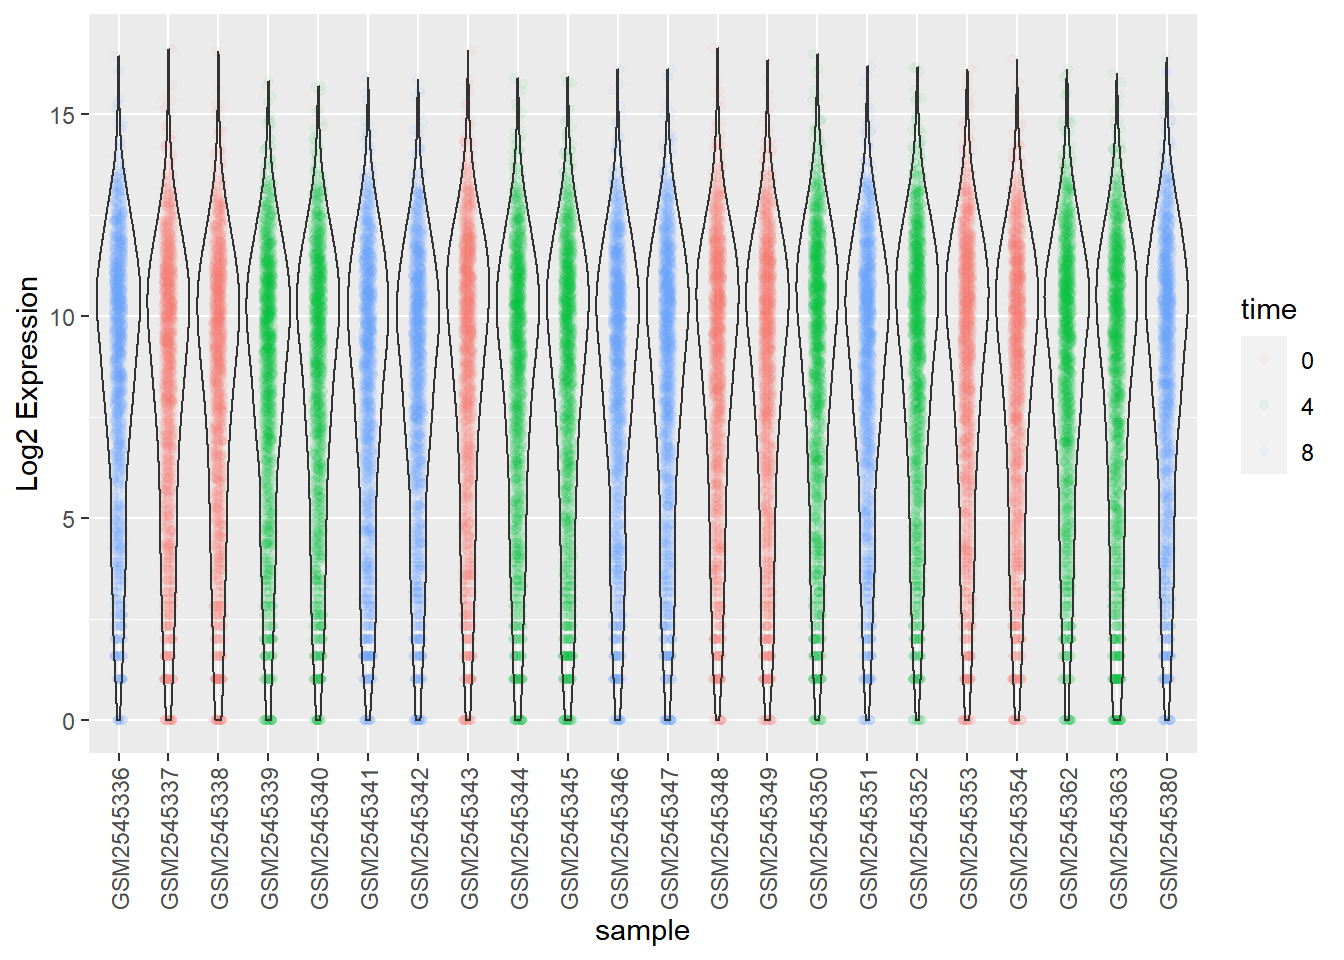
\includegraphics{Final-Machine-Learning_files/figure-latex/unnamed-chunk-13-1.pdf}

\begin{Shaded}
\begin{Highlighting}[]
\NormalTok{model }\SpecialCharTok{\%\textgreater{}\%} 
  \FunctionTok{evaluate}\NormalTok{(x\_test,}
\NormalTok{           y\_test)}
\end{Highlighting}
\end{Shaded}

\begin{verbatim}
##      loss  accuracy 
## 0.5089399 0.8672566
\end{verbatim}

\begin{Shaded}
\begin{Highlighting}[]
\DocumentationTok{\#\#prediction }
\NormalTok{pred }\OtherTok{\textless{}{-}}\NormalTok{ model }\SpecialCharTok{\%\textgreater{}\%} \FunctionTok{predict}\NormalTok{(x\_test, }\AttributeTok{batch\_size =} \DecValTok{16}\NormalTok{)}
\NormalTok{Y\_pred }\OtherTok{=} \FunctionTok{round}\NormalTok{(pred)}
\CommentTok{\# Confusion matrix}
\NormalTok{CM }\OtherTok{=} \FunctionTok{table}\NormalTok{(Y\_pred, y\_test)}

\NormalTok{CM}
\end{Highlighting}
\end{Shaded}

\begin{verbatim}
##       y_test
## Y_pred   0   1
##      0  94  13
##      1  19 100
\end{verbatim}

\end{document}
